% !TEX root = ../../presentation.tex
% Core

\begin{slide}{conversions}
\begin{tikzpicture}

% pseudo element for centering
\node (center) {};

\node (memory) 
	[font=\scriptsize, draw=black, rounded corners,  align=center, minimum height=1cm, minimum width=2cm, left=1.5cm of center] 
	{common\\ memory\\ representation\\ (LE, AS)};
	
\node (anymemory) 
	[font=\scriptsize, align=center, left=1.5cm of memory, minimum width=2cm, draw=black, rounded corners] 
	{any memory\\ representation};
	
\node (permutation) 
	[font=\scriptsize, left=0.5cm of memory, draw=black, circle] {}
      edge [<->]             (anymemory)
      edge [<->]            (memory);
      	
\node (permutation_label) 
	[font=\scriptsize, below=0.75cm of permutation] 
	{permutation};
	
\draw [->, dashed] (permutation_label) -- (permutation);
	
\node (integral) 
	[font=\scriptsize, draw=black, rounded corners,  align=center, minimum height=1cm, minimum width=2cm, right=1.5cm of center] 
	{Integral};


\node [font=\scriptsize] (toIntegral) [above=1cm of center, draw=black] {toIntegral()}
      edge [bend right, <-]            (memory)
      edge [bend left, ->]             (integral);
   
\node (signfunction) 
	[font=\scriptsize, above left=0.7cm of toIntegral] 
		{sign function};

\node (toMemoryValue) 
	[font=\scriptsize, below=1cm of center, draw=black] 
	{toMemoryValue()}
      edge [bend left, ->]             (memory)
      edge [bend right, <-]            (integral);
      
\draw [->, dashed] (signfunction) -- (toIntegral) ;
      
\end{tikzpicture}
\end{slide}


\begin{slide}{register}
  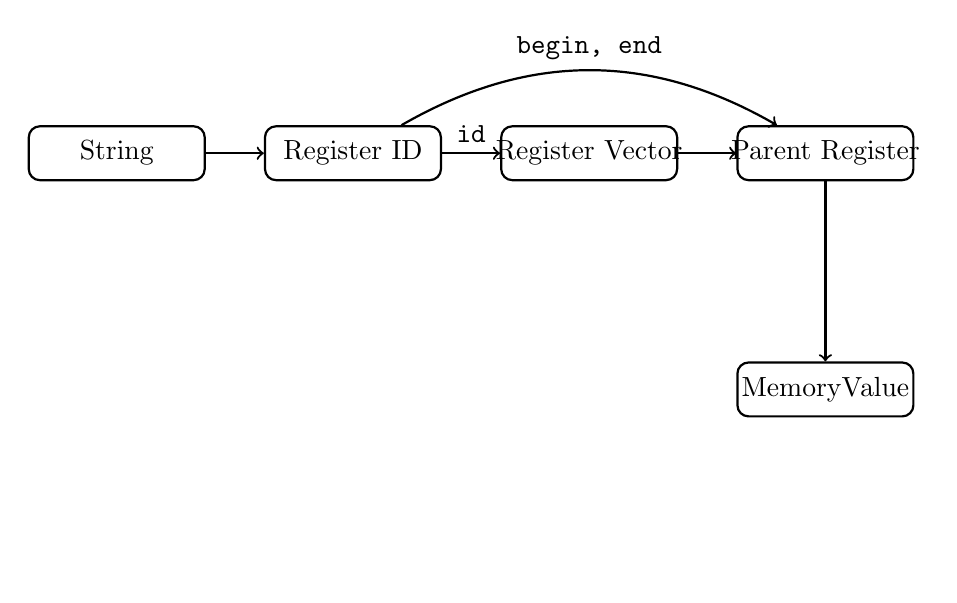
\begin{tikzpicture}[thick]

    \tikzset{block/.style={%
      draw,%
      rectangle,%
      rounded corners,%
      text width=2cm,%
      text height=0.45cm}%
    };

    \tikzset{smallblock/.style={block, text width=1.5cm, text height=0.3cm}};

    %%%%%%%%%%%%%%%
    %  register   %
    %%%%%%%%%%%%%%%
    \path (-4.5, 0) coordinate [block] (str) node {String};
    \path (-1.5, 0) coordinate [block] (rid) node {Register ID};
    \path (1.5, 0) coordinate [block] (rvc) node {Register Vector};
    \path (4.5, 0) coordinate [block] (pre) node {Parent Register};
    \path (4.5, -3) coordinate [block] (mvl) node {MemoryValue};
    \path[draw=white] (-4.5, -3) coordinate [block] (white) node {};
    \path[draw=white] (4.5, -5) coordinate [block] (white) node {};

    \draw [->] (str) -- (rid);
    \draw [->] (rid) -- (rvc) node [midway, above] {\texttt{id}};
    \draw [->] (rvc) -- (pre);
    \draw [->] (rid) to [out=30,in=150] node [midway, above] {\texttt{begin, end}} (pre);
    \draw [->] (pre) -- (mvl);

  \end{tikzpicture}
\end{slide}

\begin{slide}{register}
  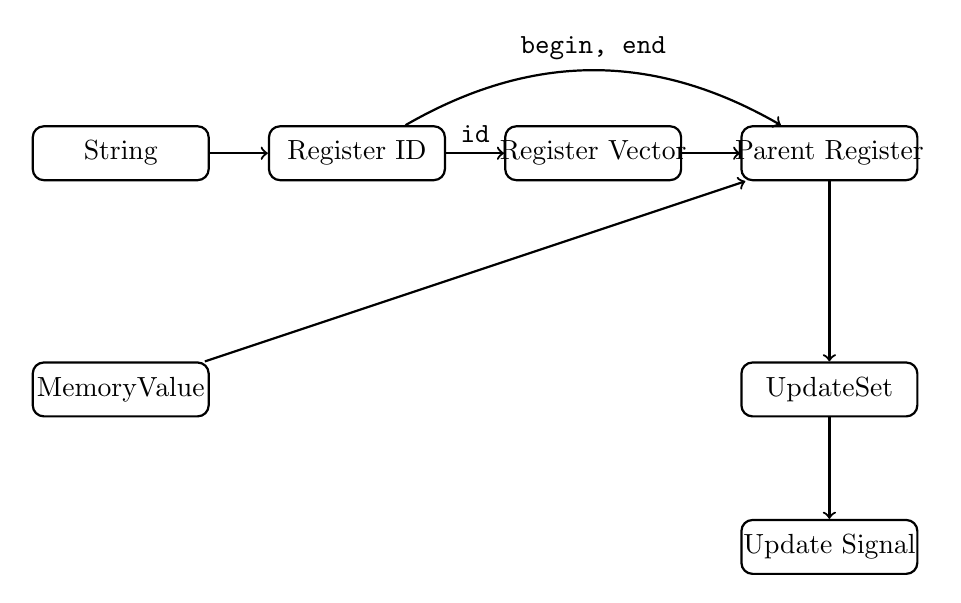
\begin{tikzpicture}[thick]

    \tikzset{block/.style={%
      draw,%
      rectangle,%
      rounded corners,%
      text width=2cm,%
      text height=0.45cm}%
    };

    \tikzset{smallblock/.style={block, text width=1.5cm, text height=0.3cm}};

    %%%%%%%%%%%%%%%
    %  register   %
    %%%%%%%%%%%%%%%
    \path (-4.5, 0) coordinate [block] (str) node {String};
    \path (-1.5, 0) coordinate [block] (rid) node {Register ID};
    \path (1.5, 0) coordinate [block] (rvc) node {Register Vector};
    \path (4.5, 0) coordinate [block] (pre) node {Parent Register};
    \path (-4.5, -3) coordinate [block] (mvl) node {MemoryValue};
    \path (4.5, -3) coordinate [block] (ups) node {UpdateSet};
    \path (4.5, -5) coordinate [block] (sig) node {Update Signal};

    \draw [->] (str) -- (rid);
    \draw [->] (rid) -- (rvc) node [midway, above] {\texttt{id}};
    \draw [->] (rvc) -- (pre);
    \draw [->] (rid) to [out=30,in=150] node [midway, above] {\texttt{begin, end}} (pre);
    \draw [->] (mvl) -- (pre);
    \draw [->] (pre) -- (ups);
    \draw [->] (ups) -- (sig);

  \end{tikzpicture}
\end{slide}

\begin{slide}{MemoryValue}
\scalebox{0.65}{
  \begin{tabular}{l|cccc}
    $\times$ & rw-single-bit & rw-single-byte & rw-subString & constructionTime-size \\
    \texttt{std::vector}\textless bool\textgreater & $\checkmark$ & $\times$ & $\checkmark$ & $\checkmark$ \\
    \texttt{boost::dynamic\_bitset} & $\checkmark$ & $\times$ & $\times$ & $\checkmark$ \\
    \texttt{std::bitset} & $\checkmark$ & $\times$ & $\times$ & $\times$ \\
    \texttt{std::vector\textless std::uint8\_t\textgreater} & $\times$ & $\checkmark$ & $\checkmark$ & $\checkmark$ \\
    \texttt{magic} & $\checkmark$ & $\checkmark$ & $\checkmark$ & $\checkmark$ \\
  \end{tabular}
  }
\end{slide}
